\section{Implementation details}

This section covers the implementation details of the developed library. It gives an insight into the selected storage formats, algorithms for GPU processing, and chosen third-party instruments for the library foundation.

\subsection{General}

Developed spla library is written using C++17 language and standard library. CMake 3.17 is used as build configuration tool. Ninja library is used to generate platform specific build files. Library supports build on Linux (tested on Ubuntu 20.04), Windows (tested on 10) and macOS (tested on Catalina). Git used as version control system. Library is compiled into shared executable object with respect to the target platform naming convention and object extension.\\

Project directory has the following structure.

\begin{itemize}[noitemsep,topsep=0pt,parsep=0pt,partopsep=0pt]
    \item \textit{include}. Public library interface files in \textit{.hpp} format. 
    \item \textit{source}. Library private source files, compiled into shared executable object.
    \item \textit{deps}. Third-party project dependencies stored as git sub-modules. 
    \item \textit{tests}. Directory with tests files for Google Tests.
    \item \textit{examples}. Example applications for graph algorithms execution.\\
\end{itemize}

\textbf{Tasking.} Taskflow~\cite{Huang2022TaskflowAL} library is utilized as a tasking library. Tasflow allows to compose the flow of the execution in a form of a task graph. Nodes inside this graph represent tasks, graph edges are dependencies between tasks. Library automatically orders tasks and schedules them to occupy all available workers. Taskflow also supports dynamic tasking and subtasks concept. Idea of these features is depicted in the figure~\ref{fig:dyn_task_flow}. It allows to add new subtasks in a time of the single task execution. This feature is utilized for processing matrices and vectors with blocked structure, when subtasks per block are spawned inside single mathematical operation.\\

\begin{figure}
    \centering
    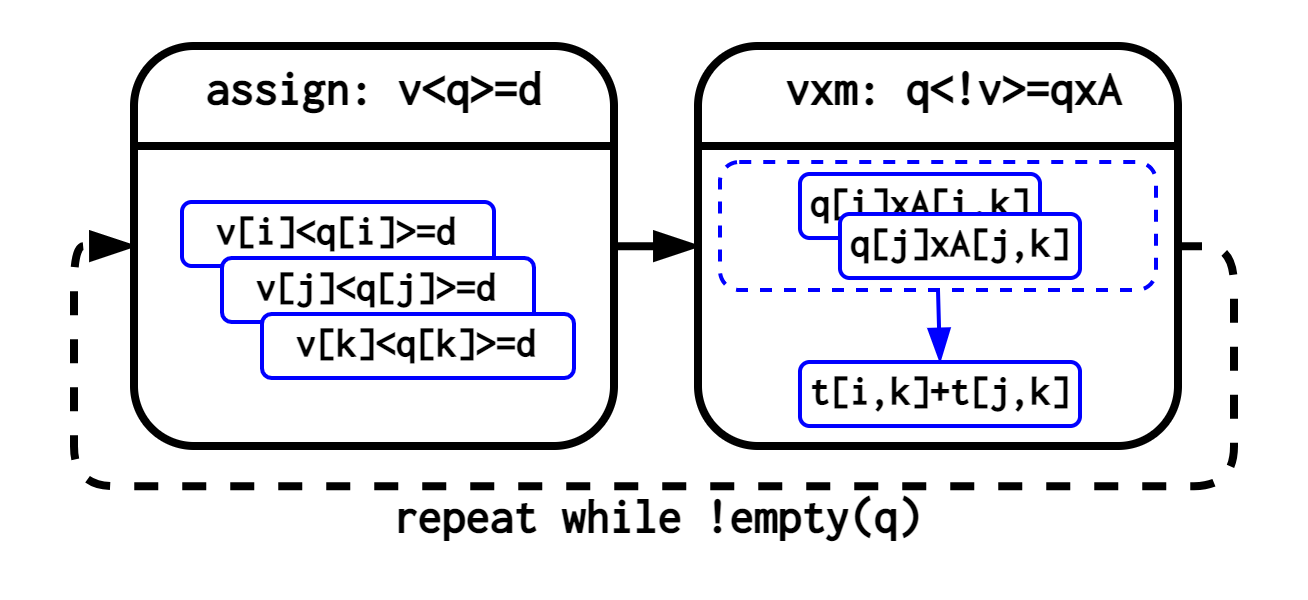
\includegraphics[width=0.9\textwidth]{images/dynamic_tasking_flow.png}
    \caption{Dynamic tasking and sub-tasks in bfs algorithms task graph for primitives with blocked structure.}
    \label{fig:dyn_task_flow}
\end{figure}

\textbf{Compute.} Boost Compute~\cite{article:boost_compute} is utilized as a OpenCL GPU computing library. Boost Compute provides C++ template-based type-safe modern high-level primitives to develop compute applications. It provides C++ wrapper for OpenCL API. It has type-safe containers, such as a \textit{vector}, \textit{map} for a device usage. Also, this library automates data read-write operations. 

Boost Compute provides \textit{meta-kernel programming} model, utilized in this work. This model allows to write OpenCL kernels in a form of a C++ template code, which is compiled and cached at runtime. This mechanism allows to write generic type and operation agnostic kernels, required to support user-defined functions and types parametrization. Meta-kernel example from the boost compute library is shown in the function \textit{set\_range} in the listing~\ref{alg:boost_meta_kernel}.

\lstset{style=codelistingstyle}

\begin{algorithm}[]
\floatname{algorithm}{Listing}
\caption{Gather meta-kernel from Boost Compute library.}
\label{alg:boost_meta_kernel}
\begin{lstlisting}[language=C++]
template<class InputIterator, class MapIterator, class OutputIterator>
class gather_kernel : public meta_kernel {
public:
    void set_range(MapIterator first, MapIterator last, 
                   InputIterator input, OutputIterator result) {
        m_count = iterator_range_size(first, last);

        *this << "const uint i = get_global_id(0);\n" 
              << result[expr<uint_>("i")] << "=" << input[first[expr<uint_>("i")]] << ";\n";
    }

    // Details omitted 
};
\end{lstlisting}
\end{algorithm}

Library provides a number of standard algorithms on the top of the meta-kernel mechanism, such as device \textit{sort}, \textit{scan}, \textit{reduce}, \textit{map}, \textit{transform}, etc. which utilized as a foundation developing sparse linear-algebra algorithms. Operations supports type and function parametrization, so it is possible to customize the type of processed data.

The library has a stable release version and it is included into latest boost SDK package. However, the project has a number of critical limitations. It has issues with memory resources flags on AMD devices. What causes time and performance drops due to unintended host and devices memory coherence. Thus, boost compute must be optimized and tested on AMD devices. Also, there is a number of issues related to the performance of the core algorithms of the project, such as sorting, scan, reduce, etc. Library has common and generic implementations of these primitives, which lose in the performance to the known state-of-the-art solutions.\\

\subsection{Data Storage}

Vector storage supports two types of blocks: sparse vector blocks in a form of non-zero indices and values lists and as a fully allocated dense vector block with additional mask, which marks which values are stored and which are not. 

Vector primitive supports explicit format convertation from sparse to dense storage. It may be useful for incremental algorithms which accumulates result, where at some moment spars blocks have more overhead compared to dense blocks usage.

Matrix storage supports blocks in list of coordinates (COO) and compressed sparse row (CSR) formats. Other storage formats, such as compressed sparse column (CSC), delta-compressed storage row (dCSR), etc., can be added by the extension of the matrix block interface. This process does not require the modification of generalized blocks grid processing. However, for each new format new combinations of algorithms must be added to the algorithm registry. 

Scalar values are stored in form of a device buffer. This values are used for \textit{reduce} and \textit{assign} operations.

\begin{figure}
    \centering
    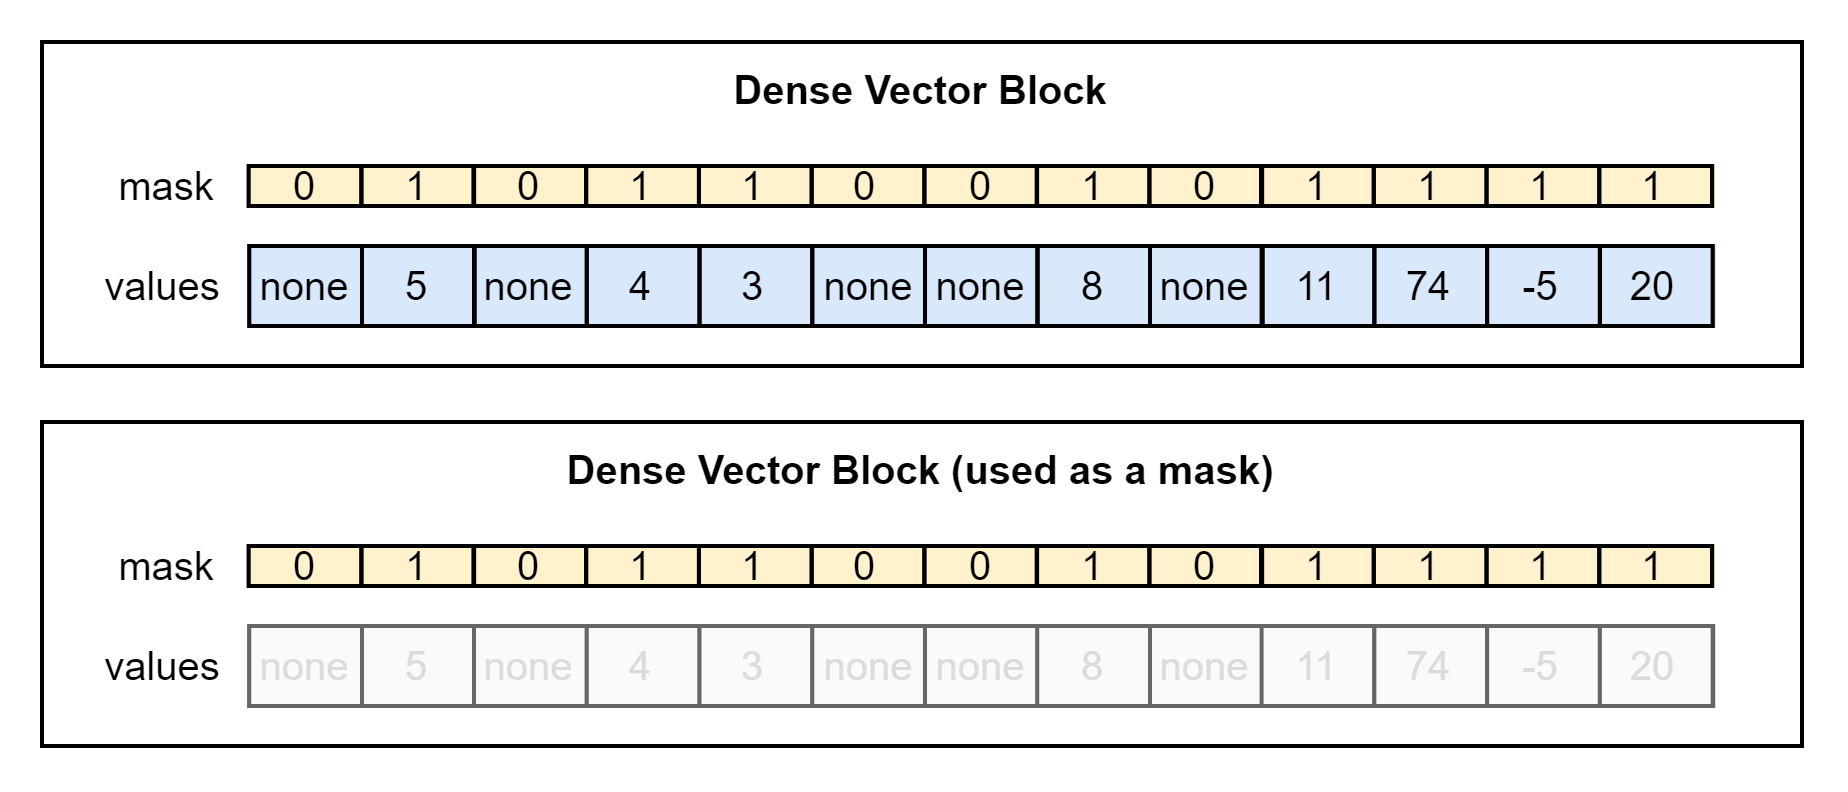
\includegraphics[width=0.8\textwidth]{images/vector_dense_block.png}
    \caption{Dense vector storage block. When used as a mask, values buffer is ignored, only mask buffer is utilized.}
    \label{fig:dense_vec_block}
\end{figure}

Matrix or vector primitives can be used as a \textit{mask} to filter the result for partial evaluation. When matrix or vector used as a mask, non-zero values are interpreted as mask values. Library explicitly stores non-zero values, so matrix or vector in any storage type can be used as a mask with loss of the flexibility as shown in the figure~\ref{fig:dense_vec_block}.

Vector and matrix blocks are immutable by default. Single vector or matrix block can be safely used in multiple operations for read operations.

\subsection{Operations}

Computational expression is constructed in a form of the DAG in the library. Nodes of the graph represent operations on matrices, vectors and scalars. Library provides a number of common and widely used operations for evaluation.

\begin{itemize}
    \item \textit{Scalar write.} Writes scalar values from user provided buffer.
    \item \textit{Scalar read.} Reads scalar value to user provided buffer.
    \item \textit{Vector write.} Writes vector data from lists of indices and values from user provided buffers.
    \item \textit{Vector read.} Reads vector data in a form of lists of indices and values to user provided buffers.
    \item \textit{Matrix write.} Writes matrix data from lists of row, column indices and values from user provided buffers.
    \item \textit{Matrix read.} Reads matrix data in a form of lists of row, column indices and values to user provided buffers.
    \item \textit{Vector assign.} Assigns a provided scalar values to a vector using structure from a mask. 
    \item \textit{Vector reduce to scalar.} Reduction of vector values using \textit{add} function to a single scalar value. Supports optional mask vector to reduce only selected values.
    \item \textit{Matrix reduce to scalar.} Reduction of matrix values using \textit{add} function to a single scalar value. Supports optional mask matrix to reduce only selected values.
    \item \textit{Vector element-wise addition.} Element-wise addition of two vectors using \textit{add} function. Supports optional mask vector to add only selected elements. 
    \item \textit{Matrix element-wise addition.} Element-wise addition of two matrices using \textit{add} function. Supports optional mask matrix to add only selected elements. 
    \item \textit{Vector-matrix product.} Classic vector-matrix product using \textit{mult} and \textit{add} functions with optional mask vector to evaluate only selected result values.
    \item \textit{Matrix-matrix product.} Classic matrix-matrix product using \textit{mult} and \textit{add} functions with optional mask matrix to evaluate only selected result values.
    \item \textit{Matrix transpose.} Transpose matrix values against main diagonal. 
    \item \textit{Matrix triangular lower.} Constructs a triangular matrix from a lower part of the original matrix below main diagonal.
    \item \textit{Matrix triangular upper.} Constructs a triangular matrix from an upper part of the original matrix above main diagonal.
\end{itemize}

% \subsection{Optimizations}

\subsection{Running example}

\lstset{style=codelistingstyle}

\begin{algorithm}[]
\floatname{algorithm}{Listing}
\caption{Breadth-first search algorithm implementation using Spla API.}
\label{alg:spla_bfs_example}
\begin{lstlisting}[language=C++]
void spla::Bfs(RefPtr<Vector> &sp_v, 
               const RefPtr<Matrix> &sp_A, 
               Index s, 
               const RefPtr<Descriptor> &descriptor) {
    float denseFactor = 1.0f;

    if (descriptor.IsNotNull()) {
        descriptor->GetParamT(Param::DenseFactor, denseFactor);
    }

    auto &library = sp_A->GetLibrary();
    auto n = sp_A->GetNrows();

    sp_v = Vector::Make(n, Types::Int32(library), library);       // Reached levels
    auto sp_q = Vector::Make(n, Types::Void(library), library);   // Bfs frontier
    auto sp_depth = Scalar::Make(Types::Int32(library), library); // Current depth

    auto sp_desc_accum = Descriptor::Make(library);
    sp_desc_accum->SetParam(Param::AccumResult);
    auto sp_desc_comp = Descriptor::Make(library);
    sp_desc_comp->SetParam(Param::MaskComplement);

    auto sp_setup = Expression::Make(library);
    sp_setup->MakeDataWrite(sp_q, DataVector::Make(&s, nullptr, 1, library));
    sp_setup->SubmitWait();

    std::int32_t depth = 1; // Start for depth 1: v[s]=1

    bool sparseToDense = false;

    while (sp_q->GetNvals() != 0) {
        auto sp_iter = Expression::Make(library);
        auto t1 = sp_iter->MakeDataWrite(sp_depth, DataScalar::Make(&depth, library));
        auto t2 = sp_iter->MakeAssign(sp_v, sp_q, nullptr, sp_depth, sp_desc_accum);
        auto t3 = sp_iter->MakeVxM(sp_q, sp_v, nullptr, nullptr, sp_q, sp_A, sp_desc_comp);

        if (!sparseToDense && sp_v->GetFillFactor() >= denseFactor) {
            auto tt = sp_iter->MakeToDense(sp_v, sp_v);
            sp_iter->Dependency(tt, t2);
            sparseToDense = true;
        }

        sp_iter->Dependency(t1, t2);
        sp_iter->Dependency(t2, t3);
        sp_iter->SubmitWait();

        depth += 1;
    }
}
\end{lstlisting}
\end{algorithm}

As an example of the developed Spla library usage consider breadth-first search algorithm implementation shown in the code listing~\ref{alg:spla_bfs_example}. 

Algorithm procedure is declared in the \textit{spla} namespace in the public interface file. The implementation of the algorithm is defined in the private cpp source file, compiled into shared object library. Procedure expects as an input reference to the result vector $v$ where to store reached depths of vertices, adjacency matrix of the graph $A$, index of the start vertex $s$ and an optional descriptor to tweak algorithm execution.

Before actual execution, parameters are read from the descriptor in liners \textbf{5 -- 9}, global library state obtained from the matrix in line \textbf{11} and graph size saved as $n$ in line \textbf{12}.

Then in lines \textbf{14 -- 16} data containers required for the algorithm execution are allocated. Vector with reached vertices as well as scalar are created with \textit{int32} type, frontier of active vertices for the search is allocated with \textit{void} type, since we are interested only in the structure of the frontier.

In lines \textbf{18 -- 21} some descriptors for expression nodes are created. Descriptor used to update reached vertices in the \textit{assign} node is configured with \textit{AccumResult} parameter. This parameter tells library, that the previous content of the result vector must be preserved and accumulated with new values. Traversal descriptor is created with \textit{MaskComplement} parameter. This parameter tells library that passed mask must be interpreted as inverted one.

Initial frontier start vertex is set in lines \textbf{23 -- 25}. Temporary expression is created and \textit{write} node used to write start index to the $q$. Since frontier has void type, index is passed without values.

The algorithm iterates in the \textit{while loop} in lines \textbf{31 -- 48} until frontier of vertices to visit is not empty. Iteration expression is construed in the lines \textbf{33 -- 35}. Firstly, the scalar is updated with new depth value. Then, this depths are assigned to the result vector using frontier as $v[q] = depth$. After assign new frontier is obtained as $q[!v] = q \times A$. Note, that vector $v$ used as inverted mask to filter all already visited vertices. In lines \textbf{37 -- 41} sparse to dense transition of the vector $v$ is done, if density factor of $v$ exceeds predefined parameter. This is an heuristic optimization done in order to reduce overhead of sparse operation in a case of very dense result.

After the execution the vector $v$ for each graph vertex stores either the depth of the vertex or nothing in the case if this vertex is not reachable from the BFS source vertex $s$. Since library API relies on C++ RAII mechanism, no explicit resources cleanup is required after the execution.

% \section{Детали реализации}

% В данной секции предлагается рассмотреть основные детали реализации библиотеки \textit{cuBool} и соответствующего ей Python-пакета \textit{pycubool}, которые были разработаны в соответствии с архитектурой, представленной в предыдущей главе.

% Разработка библиотеки осуществлялась в рамках исследовательского проекта лаборатории языковых инструментов JetBrains Research. В качестве языка программирования для реализации библиотеки используется С++, 
% так как он предоставляет механизмы для ручного управления ресурсами, 
% а также позволяет использовать язык Cuda C/C++ в рамках единого компилируемого приложения. 
% Интерфейс библиотеки реализован в виде C-совместимого API.
% Исходный код компилируется в библиотеку с разделяемым кодом \textbf{libcubool.so}, 
% которая может быть динамически загружена в конечное пользовательское приложение. 
% В качестве целевой платформы для исполнения поддерживается семейство операционных систем на базе ядра Linux.

% \subsection{Примитивы и операции}

% Основным примитивом библиотеки является разреженная матрица булевых значений, 
% которая хранится в видеопамяти видеокарты в формате \textit{CSR} (compressed sparse row), 
% который позволяет использовать $O(V + E)$ памяти для хранения матрицы смежности графа. 
% Существуют и другие форматы хранения разреженных матриц: \textit{CSC} (compressed sparse column), \textit{COO} (coordinate list) и так далее. 
% Однако CSR формат был выбран на основе результатов исследования Юсуке Нагасака и др.~\cite{inproceedings:spgemm_mem_saving_for_nvidia}, 
% так как он позволяет эффективно реализовать операцию матричного умножения в условиях ограниченного объема доступной видеопамяти. 

% В качестве поэлементных операций сложения и умножения используются \textit{логическое-или} и \textit{логическое-и}. 
% Основные функции работы с матрицами представлены ниже.

% \begin{itemize}[noitemsep,topsep=0pt,parsep=0pt,partopsep=0pt]
%     \item Создание матрицы $M$ размера $m \times n$.
%     \item Удаление матрицы $M$ и освобождение занятых ею ресурсов.
%     \item Заполнение матрицы $M$ списком значений $\{(i, j)_k\}_k$.
%     \item Чтение из матрицы $M$ списка значений $\{(i, j)~|~M[i,j]=1\}$.
%     \item Транспонирование матрицы $M = N^T$.
%     \item Извлечение подматрицы $M = N[i:k, j:t]$.
%     \item Редуцирование матрицы к вектору $V$:~$V[i]=\bigoplus_j M[i,j]$.
%     \item Сложение матриц $C \mathrel{+}= M$.
%     \item Умножение матриц $C \mathrel{+}= M \times N$.
%     \item Произведение Кронекера для двух матриц $C = M \otimes N$.
% \end{itemize}

% \subsection{Cuda-модуль}

% Операции линейной алгебры для работы с матрицами реализованы с использованием технологии Cuda. 
% В качестве основы для реализации операций умножения и сложения разреженных матриц используются результаты исследования Арсения Терехова и др.~\cite{inproceedings:cfqp_matrix_with_single_source}, оформленные в виде библиотеки \textbf{Nsparse}.
% Данная библиотека была доработана, чтобы добавить возможность динамически конфигурировать механизмы использования видеопамяти. 

% Для реализации произведения Кронекера, операций транспонирования, редуцирования и извлечения подматрицы использовались примитивы библиотеки \textbf{Thrust}.
% Данная библиотека позволяет оперировать данными в терминах высокоуровневых операций \textit{свертки}, \textit{отображения} и \textit{префиксной суммы}~\cite{net:cuda_thrust}, которые выполняются на графическом процессоре. 
% \textbf{Thrust} поставляется совместно с инструментами Cuda-разработки и не требует настройки дополнительных зависимостей.

% \subsection{Python-пакет}

% Все примитивы и операции библиотеки cuBool доступны внутри Python-пакета pycubool.
% Для публикации пакета используется стандартная инфраструктура PyPI.
% Вызов функций из \textbf{cuBool C API}, находящихся в скомпилированной библиотеке \textbf{libcubool.so}, осуществляется с помощью модуля \textbf{Ctypes}. 
% Данный модуль поставляется вместе с инфраструктурой Python и не требует настройки сторонних зависимостей. 
% Также в пакет pycubool добавлены дополнительные операции, которые облегчают использование данного инструмента и предоставляют конечному пользователю дополнительную функциональность.

% \begin{itemize}[noitemsep,topsep=0pt,parsep=0pt,partopsep=0pt]
%     \item Загрузка и сохранение матрицы в \textit{Matrix market} формате.
%     \item Экспортирование набора матриц в \textit{GraphViz} формате.
%     \item \textit{Красивая} печать матриц в текстовом виде.
%     \item Текстовые маркеры и имена матриц для отладки.
% \end{itemize}

% \subsection{Пример использования}

% \definecolor{codegreen}{rgb}{0,0.6,0}
% \definecolor{codegray}{rgb}{0.5,0.5,0.5}
% \definecolor{codepurple}{rgb}{0.58,0,0.82}
% \definecolor{backcolour}{rgb}{1.0,1.0,1.0}

% \lstdefinestyle{codelistingstyle}{
%     backgroundcolor=\color{backcolour},   
%     commentstyle=\color{codegreen},
%     keywordstyle=\color{magenta},
%     numberstyle=\tiny\color{codegray},
%     stringstyle=\color{codepurple},
%     basicstyle=\ttfamily\footnotesize,
%     breakatwhitespace=false,         
%     breaklines=true,                 
%     captionpos=b,                    
%     keepspaces=true,                 
%     numbers=left,                    
%     numbersep=5pt,                  
%     showspaces=false,                
%     showstringspaces=false,
%     showtabs=false,                  
%     tabsize=2
% }

% \lstset{style=codelistingstyle}

% \begin{algorithm}[]
% \floatname{algorithm}{Listing}
% \caption{Пример вычисления транзитивного замыкания с использованием cuBool C API}
% \label{alg:cubool_example}
% \begin{lstlisting}[language=C++]
% #include <cubool/cubool.h>

% cuBool_Status TransitiveClosure(cuBool_Matrix A, cuBool_Matrix* T) {
%     cuBool_Matrix_Duplicate(A, T);                       /* Копируем матрицу смежности А */

%     cuBool_Index total = 0;
%     cuBool_Index current;
%     cuBool_Matrix_Nvals(*T, &current);                   /* Количество ненулевых значений */

%     while (current != total) {                           /* Пока результат меняется  */
%         total = current;
%         cuBool_MxM(*T, *T, *T, CUBOOL_HINT_ACCUMULATE);  /* T += T x T */
%         cuBool_Matrix_Nvals(*T, &current);
%     }

%     return CUBOOL_STATUS_SUCCESS;
% }
% \end{lstlisting}
% \end{algorithm}

% \begin{algorithm}[]
% \floatname{algorithm}{Listing}
% \caption{Пример вычисления транзитивного замыкания с использованием пакета pycubool}
% \label{alg:pycubool_example}
% \begin{lstlisting}[language=Python]
% import pycubool

% def transitive_closure(a: pycubool.Matrix):
%     t = a.duplicate()                     # Копируем матрицу смежности А
%     total = 0                             # Количество ненулевых значений результата

%     while total != t.nvals:               # Пока результат меняется
%         total = t.nvals
%         t.mxm(t, out=t, accumulate=True)  # t += t x t

%     return t
% \end{lstlisting}
% \end{algorithm}

% В качестве примера рассмотрим проблему вычисления \textit{транзитивного замыкания} (англ. transitive closure) для некоторого ориентированного графа без меток $\mathcal{G} = \langle V, E \rangle$. Результатом вычисления транзитивного замыкания является новый граф $\mathcal{G}_{tc} = \langle V, E_{tc} \rangle$, для которого верно следующее: $e = (v,u) \in E_{tc} \iff \exists v \pi u $ в $\mathcal{G}$. Данную проблему можно решить в терминах линейной алгебры, если представить граф в виде матрицы смежности с булевыми значениями. 

% В листинге~\ref{alg:cubool_example} представлен фрагмент кода на языке C, который решает данную задачу. В качестве аргументов функция принимает матрицу смежности исходного графа, а также указатель на идентификатор, который необходимо использовать при сохранении результирующей матрицы смежности графа после транзитивного замыкания.

% В листинге~\ref{alg:pycubool_example} представлен похожий фрагмент кода, однако он уже решает поставленную в задачу на языке Python. Здесь в качестве входного аргумента используется матрица смежности графа, в качестве результата возвращается матрица смежности графа после транзитивного замыкания.
